
\section{Experimentation}
\label{sec:experimentation}

% \begin{figure}
%   \begin{center}
%   
\begin{tikzpicture}[scale=0.6]

  \small
  
  \newcommand\X{1.45*\columnwidth/8pt};
  \newcommand\YA{0pt};
  \newcommand\YB{-60pt};


  \draw[->](0*\X, \YA) -- (9*\X, \YA);
  \draw[->](0*\X, \YB) -- (9*\X, \YB);
  
  \draw[fill=white] (0*\X, \YA) node{\textbf{\textup{A}}}
  +(-5pt, -5pt) rectangle +(5pt, 5pt);
  \draw[fill=white] (0*\X, \YB)  node{\textbf{\textup{B}}}
  +(-5pt, -5pt) rectangle +(5pt, 5pt);

  % \draw ( 1*\X, \YA ) node[above]{$\mathcal{A}$};
  % \draw ( 1*\X, \YB ) node[below]{$\mathcal{B}$};

  \draw[->] ( 2*\X, \YA ) -- node[sloped, above]{$\alpha$} (3*\X, \YB);
  % node[below left]{$\mathcal{A}$};

  \draw[decorate,decoration={brace,amplitude=6pt,mirror,raise=4pt}] (3*\X,
  -5+\YB) -- node[anchor=north, yshift=-10pt]{$B_{B\alpha}$}
  (5*\X, -5+\YB);

  % \draw ( 3*\X, \YA ) node[above]{$\mathcal{C}$};

  \draw[->] ( 3*\X, \YB ) -- node[sloped, above]{$\beta$} (4*\X, \YA);
  % node[above left]{$\mathcal{B}$};

  \draw[decorate,decoration={brace,amplitude=6pt,raise=4pt}] (4*\X,
  5+\YA) -- node[anchor=south, yshift=10pt]{$B_{A\beta} \bm{= B_{A\alpha}}$}
  (6*\X, 5+\YA);

  \draw[decorate,thick,decoration={brace,amplitude=6pt,raise=4pt}] (6*\X,
  5+\YA) -- node[anchor=south, yshift=10pt]{$\bm{B_{A\pi}}$}
  (8*\X, 5+\YA);
  
  
  % \draw ( 4*\X, \YB ) node[below]{$\mathcal{D}$};

  \draw[->] ( 4*\X, \YA ) -- node[sloped, above]{$\pi$} (5*\X, \YB);
  % node[below left]{$\mathcal{C}$};

  \draw[decorate,decoration={brace,amplitude=6pt,mirror,raise=4pt}] (5*\X,
  -5+\YB) -- node[anchor=north, yshift=-10pt]{$B_{B\pi} \bm{= B_{B\beta}}$}
  (7*\X, -5+\YB);


  % \draw ( 5*\X, \YA ) node[above]{$\mathcal{E}$};

  \draw[->] ( 5*\X, \YB ) -- node[sloped, above]{$\rho$} (6*\X, \YA);
  % node[above left]{$\mathcal{D}$};
  
  % \draw (6*\X, \YB) node[below]{$\mathcal{F}$};

  \draw[->, dashed] ( 6*\X, \YA ) -- node[sloped, above]{$B_{A\beta}$} (7*\X, \YB);

  \draw[->, dashed, thick] ( 7*\X, \YB ) --
  node[sloped, below]{$\bm{B_{B\beta}}$} (8*\X, \YA);

%  node[below left]{$\mathcal{E}$};


\end{tikzpicture}

%%% Local Variables:
%%% mode: latex
%%% TeX-master: "../paper"
%%% End:

%   \caption{\label{fig:bibroadcast}\RPCBROADCAST ensures the safety of bidirectional links
%     at marginal cost. Process~A maintains an additional buffer. Process~B transmits its
%     second buffer.}
%   \end{center}
% \end{figure}

% When links are bidirectional, \RPCBROADCAST must ensure their safety
% in both directions. Instead of performing twice \RPCBROADCAST's
% operation, we extend its behavior to handle bidirectional safety at
% once. Some control messages serve two purposes. For instance, control
% messages $\beta$ are also control messages $\alpha$. Some buffers have
% two purposes. For instance, the buffer $B_\beta$ of the process adding
% a link is also a buffer $B_\alpha$.  Figure~\ref{fig:bibroadcast}
% depicts the small change in the operation of \RPCBROADCAST. It ensures
% safety of bidirectional links at marginal cost compared to its
% unidirectional version. The buffer $B_\beta$ of Process~A becomes its
% buffer $B_\alpha$. The buffer $B_\pi$ of Process~B becomes a buffer
% $B_\beta$ that will be sent using the new link upon receipt of the
% buffer of Process~A. Between the sending of its buffer and the receipt
% of the buffer of Process~B, Process~A maintains an additional buffer
% $B_\pi$. \TODO{Maybe move this in proposal?}


\begin{figure}
  \begin{center}
    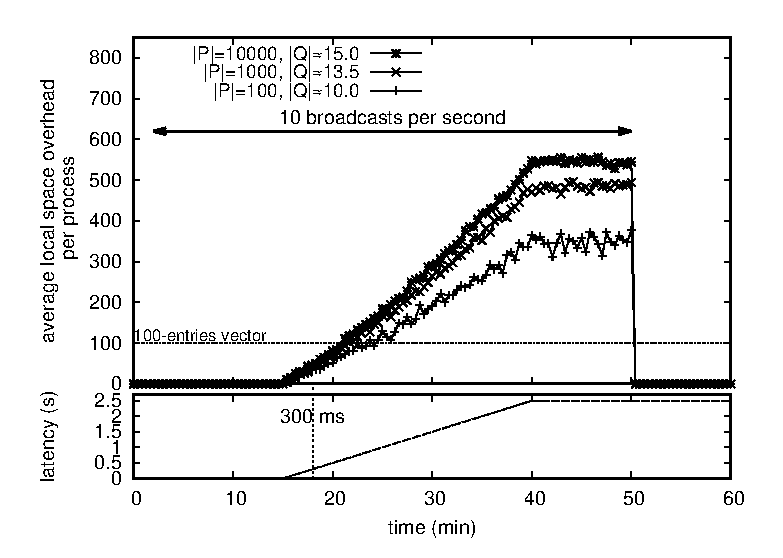
\includegraphics[width=0.8\columnwidth]{./img/overhead.eps}
    \caption{\label{fig:overhead}Local space overhead over time consumed by \RPCBROADCAST to ensure
      causal order and forbid double delivery in dynamic systems with varying latency.}
  \end{center}
\end{figure}


\noindent \textbf{Objective:} To confirm that local space complexity
depends on inviews and message receipts.

\noindent \textbf{Description:} We measure the average size of
buffers. This constitutes the average local space overhead consumed by
\RPCBROADCAST to detect and forbid double delivery in dynamic systems.
\begin{equation*}\centering\sum\limits_{p \in P} {|D_A| + |B_{A\alpha}| + |B_{A\beta}|
    + |B_{A\pi}|\over{ |P|}}
\end{equation*}
Runs involve 2 overlay networks comprising 100, and 1k
processes. \SPRAY (\REF) builds the overlay networks by providing and
maintaining neighborhoods logarithmically scaling with the number of
processes in the system. Each process of the 100-processes system has
a neighborhood of ~10.5 neighbors. Each process of the 1k-processes
system has a neighborhood of ~13 neighbors. Each process dynamically
re-configure their neighborhood every minutes by exchanging safe links
with a chosen neighbor: it gives half of its safe links to the chosen
neighbor; the latter gives half of its safe links to the former as
well. Each exchange leads to safety checks of new links and removal of
given links. \TODO{Thus, \SPRAY builds highly dynamic overlay networks
  that allows to balance the load of broadcast among processes, is
  resilient to random crashes.}\\ Links have transmission delay, i.e.,
the time between the sending of a message and its receipt is not
null. The experiments start with $1ms$ delay. At $15min$ the delay
starts to increases. At ~$17min$ links reach $300ms$ delay. At $40min$
links reach $2.5s$ delay and it stops increasing.\\ Random processes
start broadcasting messages at a rate of 10 broadcasts per second from
$2min$ to $50min$.

\noindent \textbf{Results:} Figure~\ref{fig:overhead} shows the result
of this experiment. The x-axis denotes the time in minute. The top
part of the figure shows local space overhead while the bottom part of
the figure shows the evolution of transmission delays.
\begin{itemize}
\item Figure~\ref{fig:overhead} confirms that the local space
  consumption depends on the inview size. Systems with larger inviews
  consume more space. Each new delivered message adds control information on
  each link of the inview (see Algorithm~\ref{algo:reliablebroadcast}).
\item Figure~\ref{fig:overhead} confirms that the local space
  consumption depends on network condition. The overhead increases as
  the latency increases. Latency increases the time between the first
  and the last receipt of each message. Processes store messages
  longer until they can be safely removed.
\item Figure~\ref{fig:overhead} confirms that the local space
  consumption depends on broadcast messages. When processes stops
  broadcasting, the space consummed at each process drops to 0. Each
  process eventually receive each message and safely remove the
  corresponding entry.
\item Figure~\ref{fig:overhead} shows that at a rate of 10 broadcasts
  per second and when latency stays under a realistic bound ($300ms$),
  the overhead is lower than vector-based approaches (\REF). Whatever
  system conditions, it would require a vector of 100, 1k entries to
  forbid double delivery in the 100-processes systems and 1k-processes
  system respectively.
\end{itemize}

\noindent Overall, the overhead of \PCBROADCAST depends on the system
at a given time while the overhead vector-based approaches (\REF)
depends on past messages that increases monotonically.




%%% Local Variables:
%%% mode: latex
%%% TeX-master: "../paper"
%%% End:
